\documentclass[a4paper]{article}
\usepackage[polish]{babel}
\usepackage[utf8]{inputenc}
\usepackage{polski}
\usepackage[T1]{fontenc}
\frenchspacing
\usepackage{indentfirst}
\usepackage{graphicx}
\graphicspath{{pictures/}}

\begin{document}
\maketitle

\section{Patrick Bajorski}
\label{sec:Patrick Bajorski}

\subsection{Przykładowe listy}
\begin{enumerate}
\item C
\item C++
\item Python
\item Java
\end{enumerate}

\begin{itemize}
\item Lewis Hamilton
\item Max Verstappen
\item Charles Leclerc
\end{itemize}

\subsection{Zdjęcie}
\begin{figure}[h]
    \centering
    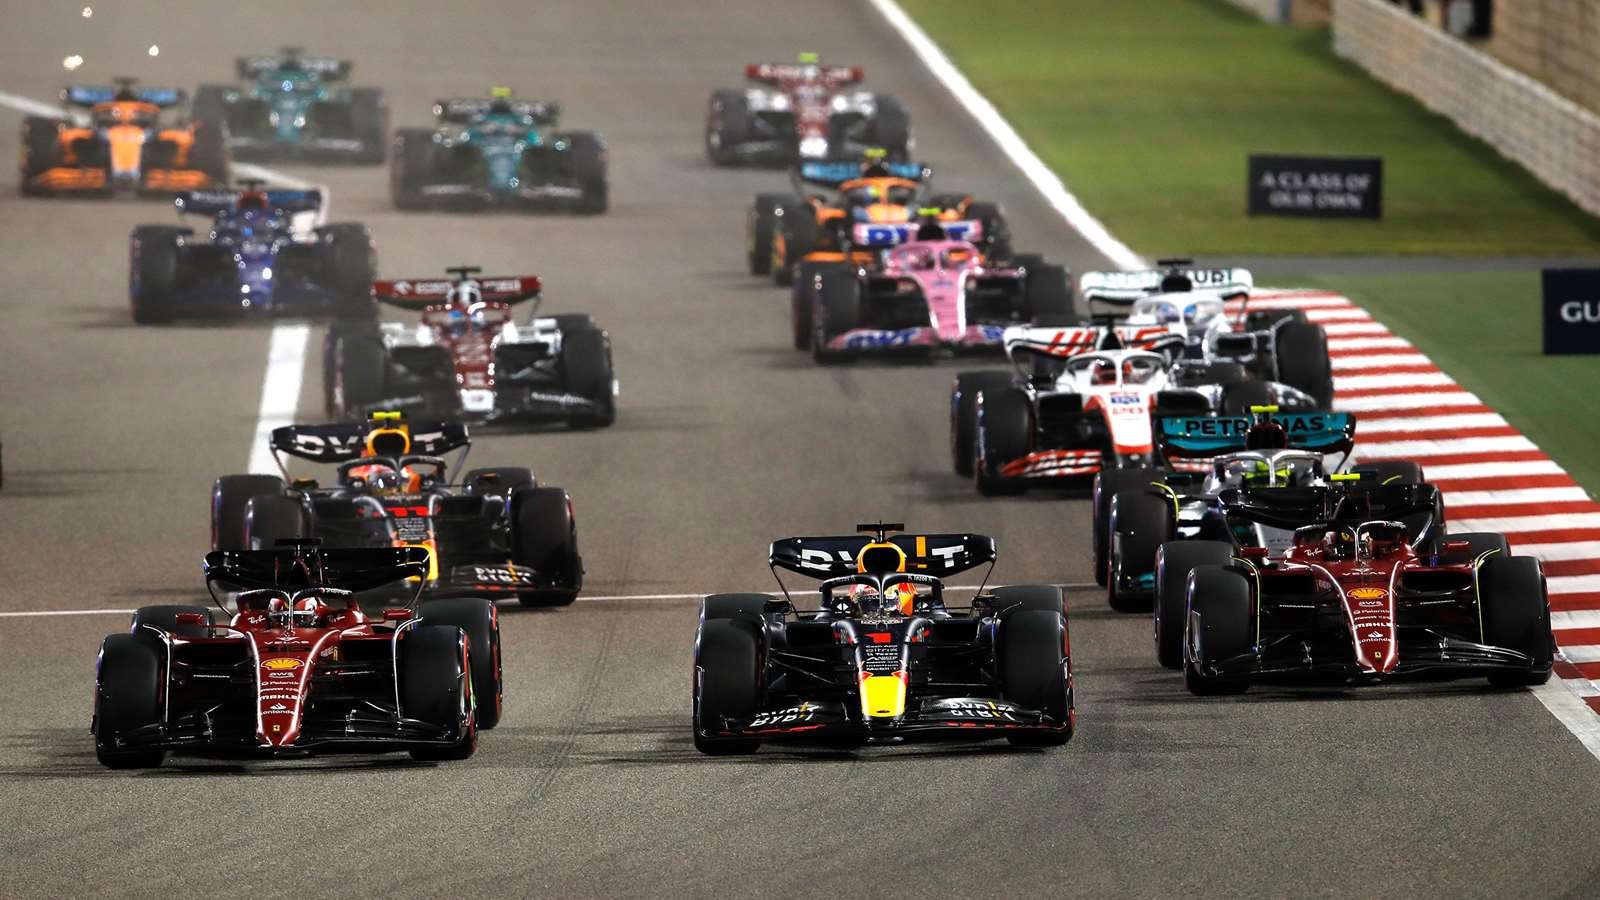
\includegraphics[width=0.75\textwidth]{pictures/F1.jpg}
    \caption{To jest zdjęcie prezentujące bolidy Formuły 1.}
    \label{fig:F11}
\end{figure}
\textit{Zdjęcie \ref{fig:F11} zostało zrobione podczas Grand Prix Bahrajnu w sezonie 2022.} \\ Było to pierwsze Grand Prix po wprowadzeniu nowych przepisów technicznych. \\ Zwycięzcą GP Bahrajnu został \emph{Charles Leclerc} z zespołu \textbf{Ferrari}

\subsection{Wyrażenie matematyczne}
\textit{Jednym z podstawowych zagadnień matematycznych jest ciąg.\\}
\huge Oto równanie przykładowego ciągu:
\[ X^{}_{n} = X^{}_{1} + X^{}_{2} + \dots + X^{}_{n} \]

\subsection{Tabela}
Ta tabela jest przykładową tabelą złożoną z
\MakeUppercase{2 kolumn oraz 2 wierszy\\}
\begin{table}[h]
\centering
\begin{tabular}{|l|l|}
\hline
Litery & Cyfry \\
\hline
a      & 1     \\
\hline
b      & 2     \\
\hline
\end{tabular}
\label{tab:PB}
\caption{Przykładowa tabela}
\end{table}

\end{document}